\subsubsection{Pitch Interpolation Evaluation}
\paragraph{Measurement Setup}

To evaluate interpolation quality (implementation details in Section \ref{sec:focus-1-pitch-interpolation}), a \qty{100}{Hz} sawtooth wave was loaded into the tape record buffer. 
A sawtooth wave was chosen as the test signal because it contains all integer harmonics (both even and odd), providing a rich spectrum of overtones across the audio band for evaluating the FFT output. \cite[p.~665]{georgearfkenMathematicalMethodsPhysicists1985}

The two interpolation methods under comparison were ZOH and the 4-point cubic Hermite 
with Catmull-Rom tangents. Each method was recorded separately at the following playback 
speeds: $0.25\times$ ($-2$ octaves), $0.33\times$, $0.5\times$ ($-1$ octave), 
$0.75\times$, $1.0\times$ (unity), $1.5\times$, $2.0\times$ ($+1$ octave), and 
$4.0\times$ ($+2$ octaves).

To eliminate possible parameter jitter and value inaccuracy from the ADC, the playback speed was fixed at compile 
time via a macro in \texttt{project\_config.h}, bypassing the control interface entirely:

\begin{minted}[linenos]{c}
#define CONFIG_TAPE_PITCH_OV~ERRIDE 4.0f
\end{minted}

The output was captured at $f_s = \qty{48}{kHz}$ as 24-bit \texttt{.wav} files 
using a professional RME Fireface UFX\,II audio interface.

\paragraph{Results}

Figure~\ref{fig:interpolation_linear_vs_zoh_fft} shows the FFT magnitude spectra of 
the recorded signals for each playback speed. 

At unity playback ($1.0\times$), both methods produce nearly identical spectra: the 
harmonic series of the sawtooth is clearly visible with no significant aliasing, as no 
interpolation is required when the playhead advances at exactly one sample per output step.

As the playback speed decreases below $1.0\times$, the effective upsampling ratio 
increases and the interpolator is called more frequently, making its quality increasingly 
audible. At $0.5\times$ and below, ZOH shows clearly visible aliasing humps between the 
signal harmonics, caused by folded spectral energy from above Nyquist. At $0.25\times$, a second 
aliasing hump appears, consistent with the broad sidelobe structure predicted by the ZOH 
frequency response in Section~\ref{sec:interpolation-comparision-frequency-response}.

The Hermite interpolator shows substantially lower aliasing across all upsampling 
ratios. Even at $0.25\times$, where ZOH produces prominent aliasing humps, the Hermite 
output retains only a small residual artefact, consistent with the suppressed sidelobe 
structure of the Catmull-Rom kernel discussed in 
Section~\ref{sec:interpolation-comparision-frequency-response}.

\begin{figure}[H]
	\centering
	\makebox[\textwidth][c]{%
		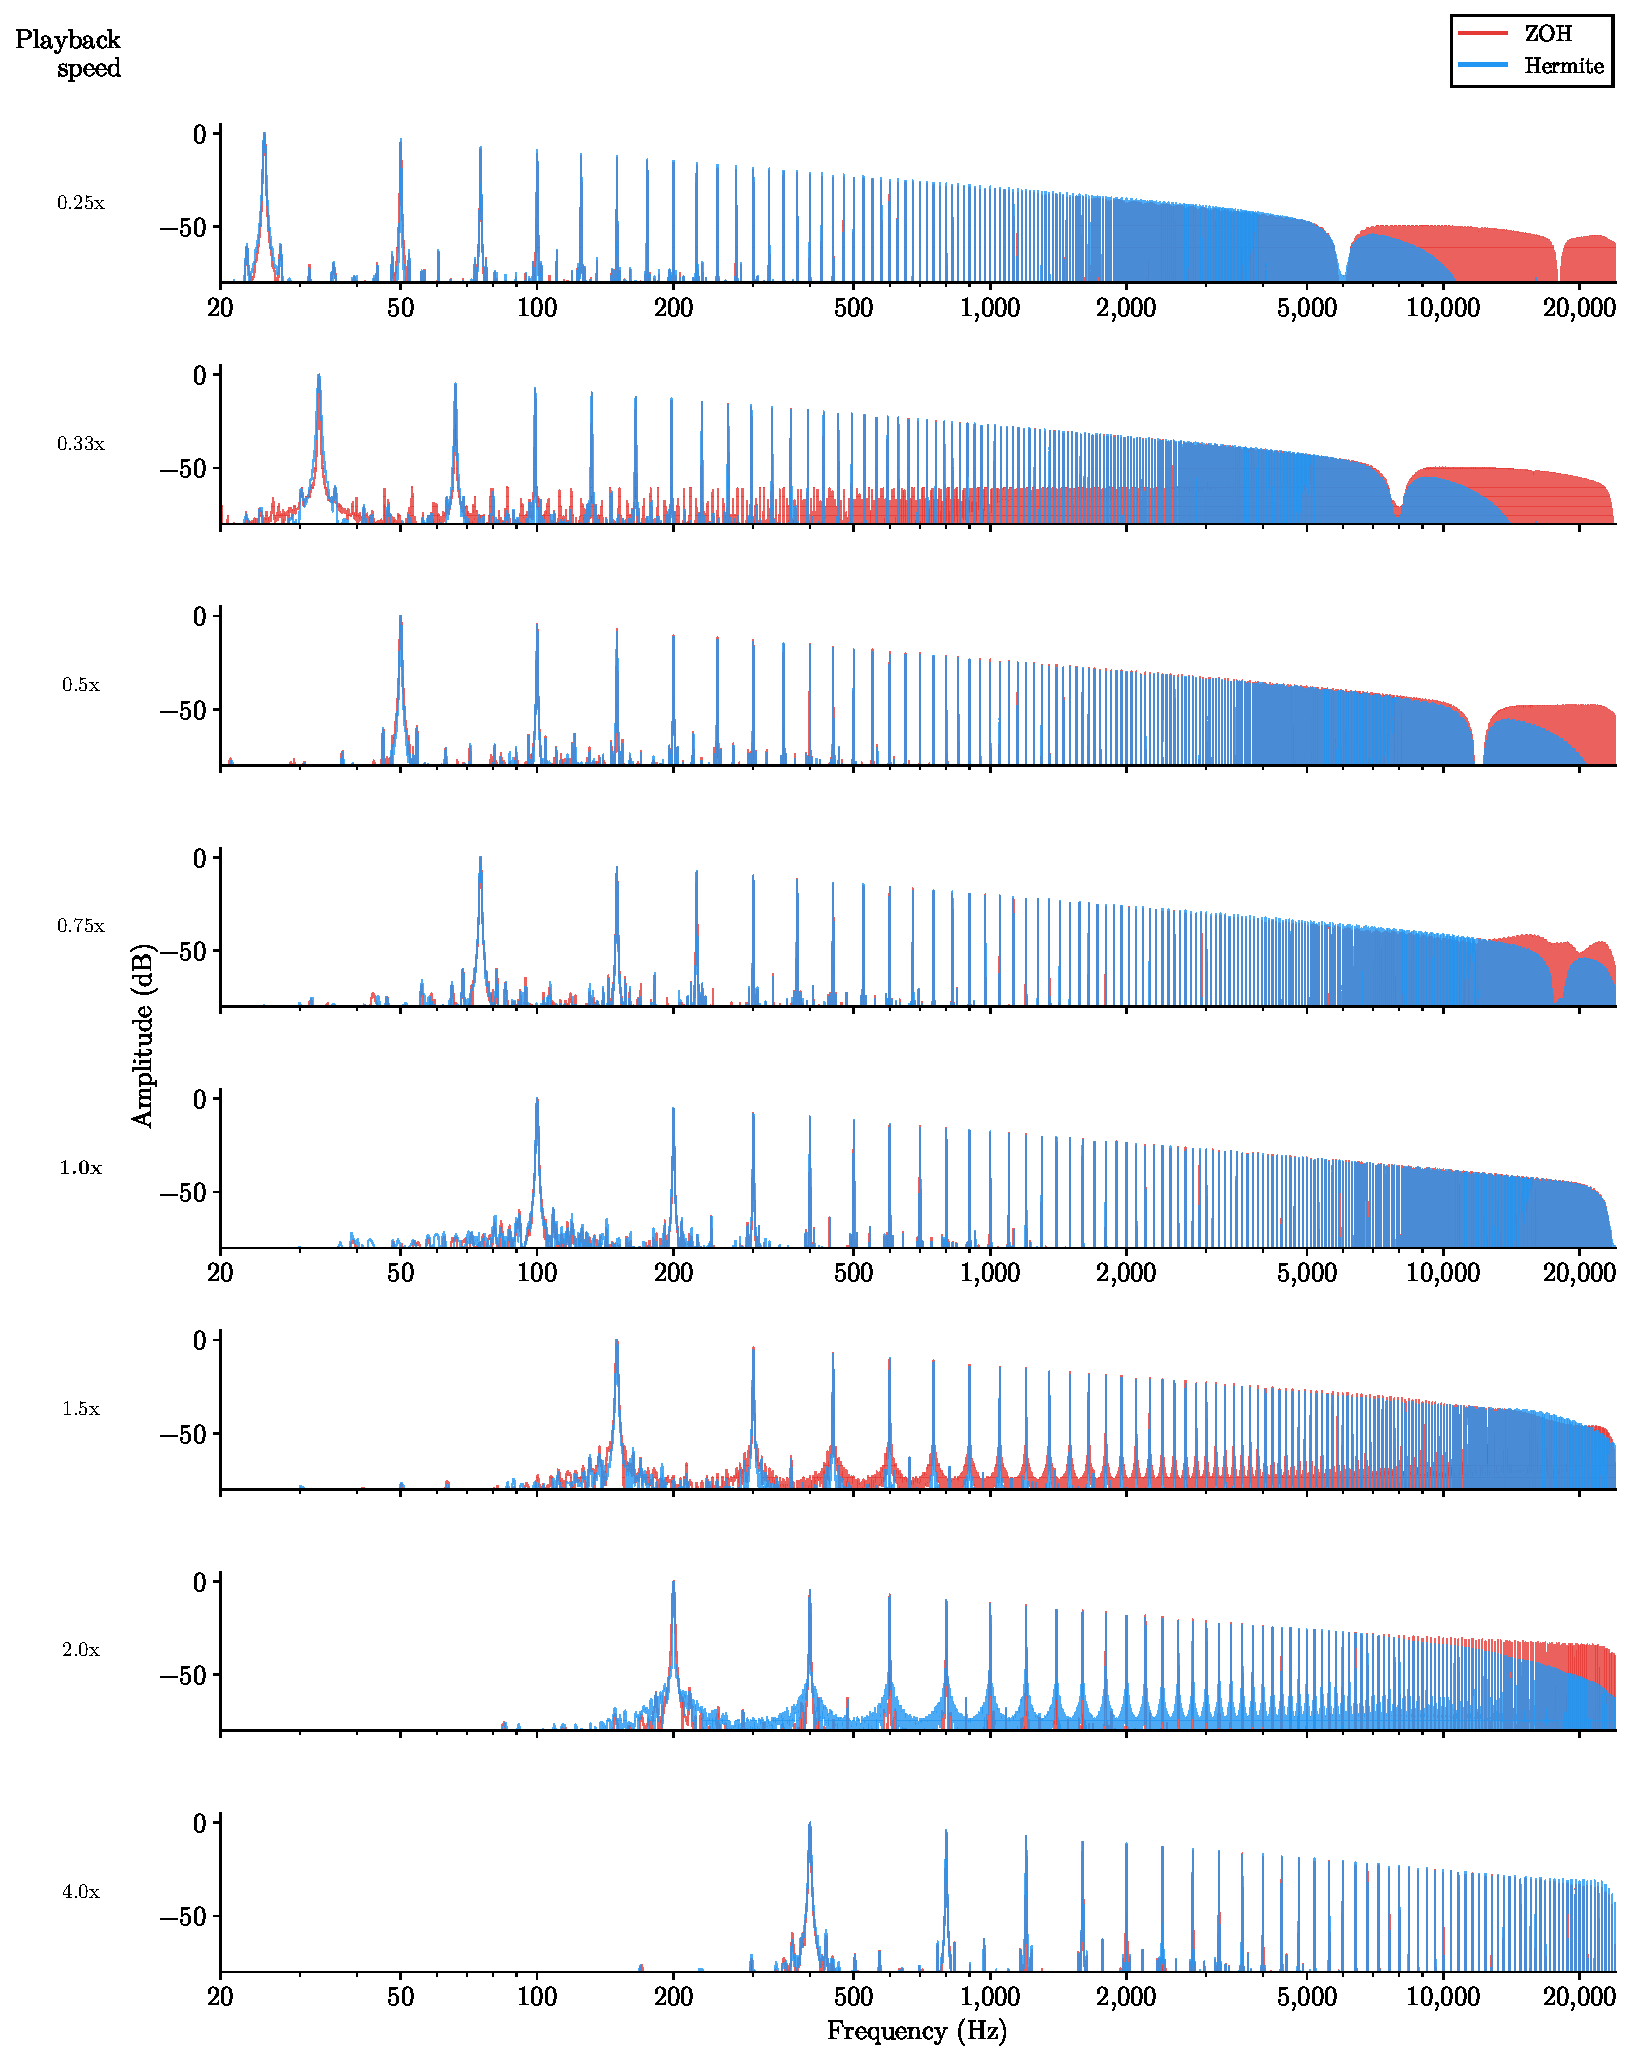
\includegraphics[width=1.0\textwidth]{../images/interpolation/fig_interpolation_fft.pdf}
	}
	\caption{FFT of 100Hz Saw signal - interpolated via Hermite and ZOH with different playback speeds}
	\label{fig:interpolation_linear_vs_zoh_fft}
\end{figure}

The qualitative comparison in Table~\ref{tab:interpolation_aliasing_comparison} 
shows the superior interpolation quality and reduced aliasing of the implemented 
cubic Hermite interpolation, at the cost of attenuation in the upper frequency 
range. For standard playback (no decimation during recording), cubic Hermite interpolation is therefore used exclusively.

\begin{table}[H]
	\centering
	\begin{tabular}{lp{3.5cm}p{4.5cm}}
		\toprule
		\textbf{Playback Speed} & \textbf{ZOH} & \textbf{Hermite (Catmull-Rom)} \\
		\midrule
		$4.0\times$ ($+2$ oct)   & Clean & Clean \\
		$2.0\times$ ($+1$ oct)   & Clean & Clean \\
		$1.5\times$              & Clean & Clean \\
		$1.0\times$ (unity)      & Clean & Clean \\
		$0.75\times$             & Minor aliasing & Clean \\
		$0.5\times$  ($-1$ oct)  & Visible aliasing humps & Minor aliasing \\
		$0.33\times$             & Strong aliasing & Minor aliasing \\
		$0.25\times$ ($-2$ oct)  & Strong aliasing, double hump & Residual artefact only \\
		\bottomrule
	\end{tabular}
	\caption{Qualitative comparison of aliasing artefacts at each playback speed.}
	\label{tab:interpolation_aliasing_comparison}
\end{table}


\subsubsection{Schroeder Reverb Evaluation}

\paragraph{Impulse Response Decay}

Figure~\ref{fig:schroeder_env_decay_measurement} shows the measured envelope decay 
of the reverb unit -- as implemented in Section \ref{sec:schroeder-reverb} -- under varying feedback and room size parameters. Each curve 
represents the smoothed amplitude envelope of a 20\,ms white noise burst passed 
through the reverb and plotted until the signal 
reaches $-60$\,dB.

\begin{figure}[H]
	\centering
	\makebox[\textwidth][c]{%
		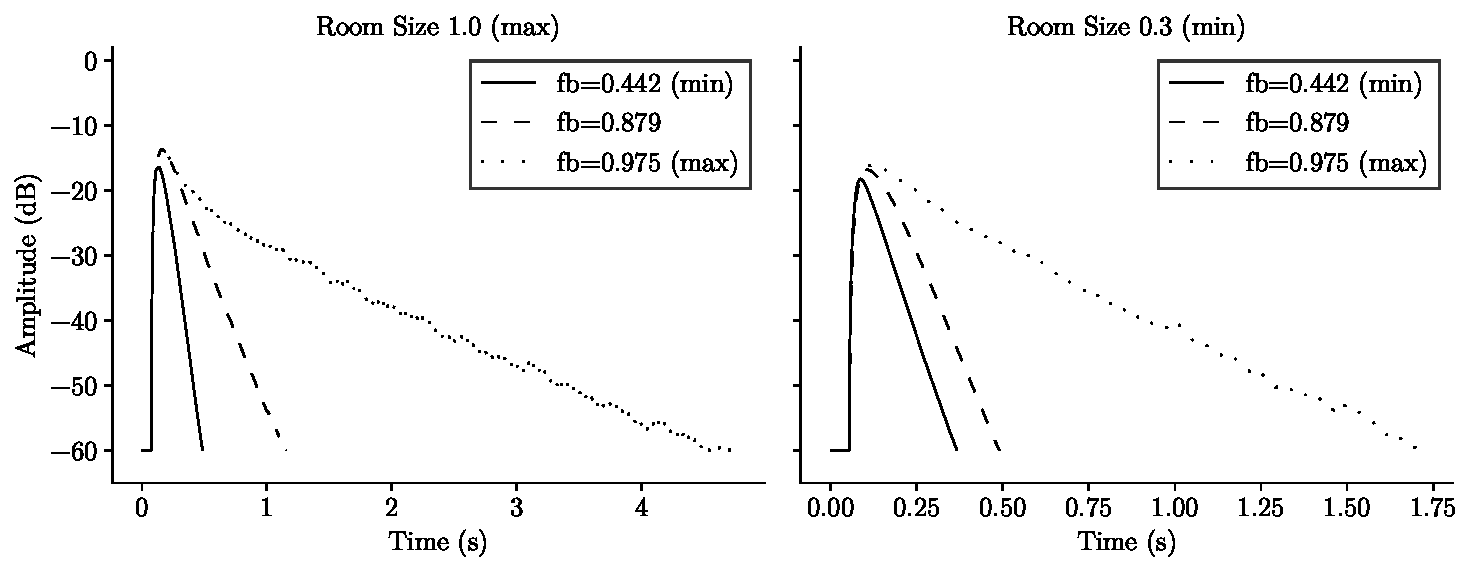
\includegraphics[width=1.0\textwidth]{../images/schroeder_reverb/fig_reverb_envelope.pdf}
	}
	\caption{Reverb Decay Times of a \qty{20}{ms} White Noise Burst}
	\label{fig:schroeder_env_decay_measurement}
\end{figure}

\paragraph{Feedback and Room Size} As expected, higher feedback coefficients result in longer decay times. 
At maximum feedback ($fb = 0.975$), the reverb tail extends significantly longer than at minimum feedback ($fb = 0.442$), which decays rapidly toward the noise floor. 
The most important validation is the stability at maximum feedback, on both maximum and minimum room sizes.

The room size parameter scales the delay line lengths of 
the comb filters. At maximum room size, the decay is smoother and more diffuse, 
while at minimum room size the shorter delay lines produce a denser, more colored 
decay. \\


The parameter boundaries were determined empirically during testing, chosen to represent the range that produces the most musically useful results (long, dense decay at the upper end and short, subtle ambience at the lower end) while ensuring the filters remain stable throughout.
\paragraph{RT60} The \qty{-60}{dB} decay time (RT60) can be read directly from the 
x-axis. At maximum feedback and room size, the RT60 is approximately \qty{5}{s}, while at minimum feedback it falls below \qty{0.5}{s}. 
Notably, at minimum room size the RT60 reaches only approximately \qty{3.25}{s} even at maximum feedback, significantly shorter than the \qty{5}{s} observed at maximum room size.
During testing, it became clear that feedback scaling (described in Section~\ref{sec:schroeder_parameter_coupling}) alone cannot fully compensate
for the shorter decay at smaller room sizes, since increasing feedback further risks
instability before the RT60 of larger room sizes can be matched.

\paragraph{Spectrogram}

Figure~\ref{fig:schroeder_env_spectrogram} shows the spectrogram of the reverb tail 
at maximum feedback ($fb = 0.975$, size $= 1.0$), comparing the comb filter lowpass 
enabled and disabled. The input is a \qty{20}{ms} white noise burst, plotted over 
\qty{5}{s} of decay.


\begin{figure}[H]
	\centering
	\makebox[\textwidth][c]{%
		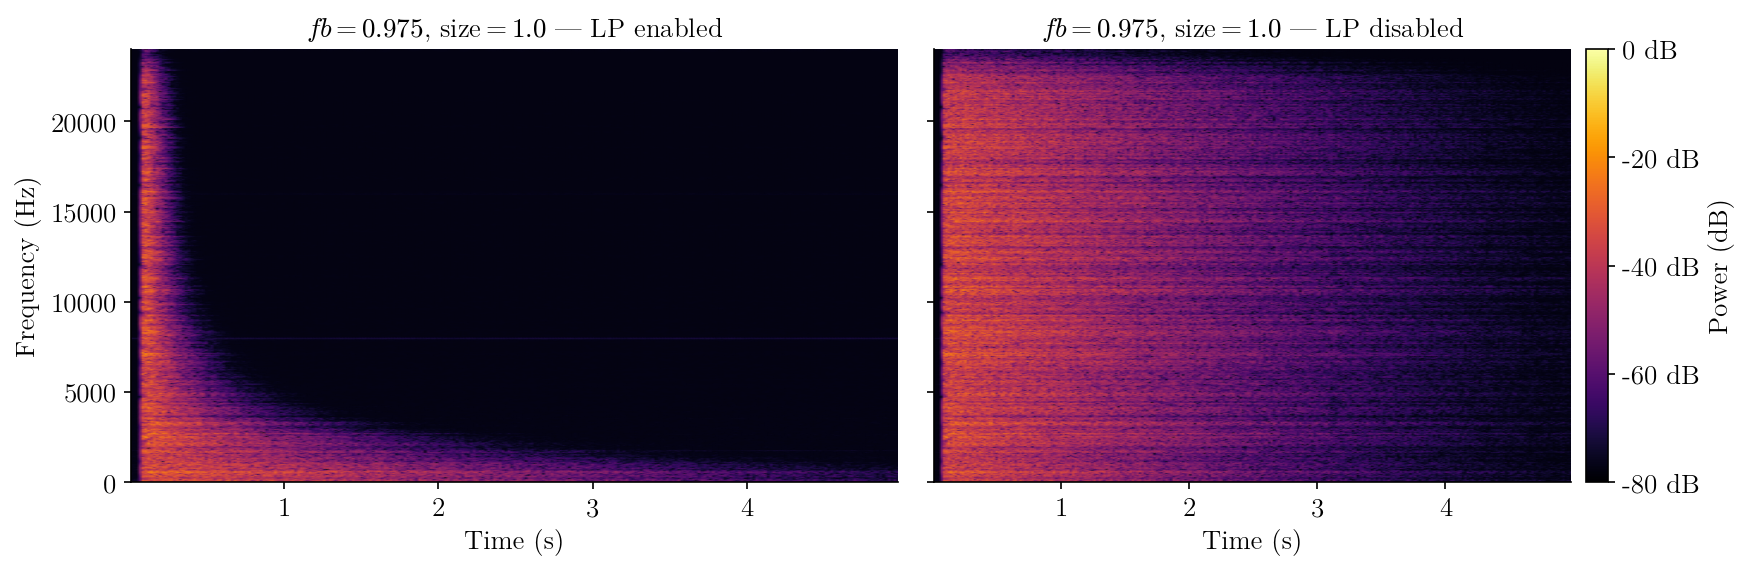
\includegraphics[width=1.0\textwidth]{../images/schroeder_reverb/fig_reverb_spectrogram.png}
	}
	\caption{Reverb Tail Spectrogram at comb lowpass filter on feedback settings}
	\label{fig:schroeder_env_spectrogram}
\end{figure}

\subparagraph{LP enabled} With the lowpass active ($d = 0.4$), high-frequency energy 
decays significantly faster than low-frequency content. The rolloff is clearly visible 
as the bright energy concentrates toward the lower frequencies over time, producing 
the characteristic warm, darkening tail associated with natural room acoustics.

\subparagraph{LP disabled} Without lowpass damping, energy is distributed more evenly 
across the frequency spectrum throughout the decay, resulting in a brighter and more 
unnatural sounding tail.

\subparagraph{Summary} Both variants have usable applications in music production. 
Engaging the lowpass produces a more natural sounding reverb tail, modelling the 
frequency-dependent absorption of a natural acoustic space, where high frequencies 
are absorbed more rapidly than low frequencies.\\

An interesting observation is that the frequency content of the reverb tail extends 
almost to the Nyquist limit of $f_s / 2$ (\qty{24}{kHz}), confirming that neither 
the used audio interface (RME Fireface UFX\,II interface \cite{FirefaceUFXII}) nor the embedded system 
introduce any significant bandlimiting, and the observed high-frequency content 
reflects the true output of the reverb algorithm.

\subsubsection{Timing and Latency Analysis}

\paragraph{Measurement Setup}

The end-to-end latency of the tape player engine was measured from gate signal 
input to audio output. A gate signal was applied to the play input and the 
resulting audio output was captured simultaneously on a two-channel oscilloscope. 
To provide sharp signal edges suitable for precise timing measurement, the fade-in, 
fade-out, and amplitude envelope were disabled for the duration of the measurement by commenting out the implemented feature-enable macros in \texttt{project\_config.h}:

\begin{minted}{c}
// #define CONFIG_ENABLE_ENVELOPE
// #define CONFIG_TAPE_PLAYER_ENABLE_FADE_IN_OUT
\end{minted}

The measurement captures the full latency chain: gate detection, FreeRTOS task 
notification, command queue processing, tape player FSM transition, DMA buffer 
output, and codec output stage.

Multiple oscilloscope captures were taken to characterise both the average latency 
and the worst-case jitter introduced by the block-based command processing.

\paragraph{Expected Latency}

With a sample rate of $f_s = \qty{48}{kHz}$ and a DMA half-block size of 64 
samples, the theoretical baseline latency and maximum deviation are:

\begin{align*}
	t_{\text{block}}         &= \frac{64}{48000} = \qty{1.333}{ms} \\
	t_{\text{min}}           &= 2 \times t_{\text{block}} = \qty{2.667}{ms} \\
	t_{\text{max}}           &= t_{\text{min}} + t_{\text{block}} = \qty{4.000}{ms} \\
	\Delta t_{\text{jitter}} &= t_{\text{block}} = \qty{1.333}{ms}
\end{align*}

The realtime latency requirement of $< \qty{5}{ms}$ (Section~\ref{sec:system-requirements}) is 
therefore expected to be met in all cases.

\paragraph{Results}

Figure~\ref{fig:latency_osc} shows oscilloscope captures of the gate-in to 
audio-out timing. Channel 1 (yellow) is the audio output signal, Channel 2 (blue) 
is the gate/play signal.

\begin{figure}[H]
	\centering
	\begin{minipage}{0.49\textwidth}
		\centering
		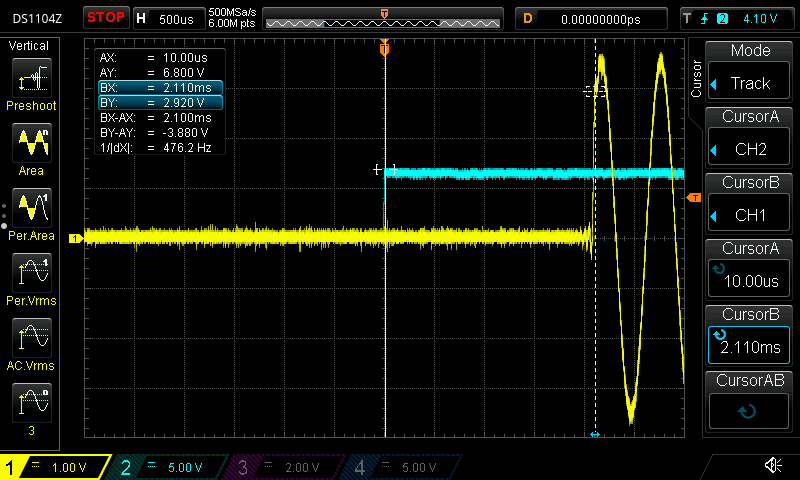
\includegraphics[width=\textwidth]{../images/signal_tests/gate-in_audio_out_latency_tape_enabled/gate-in_audio-out_latency_tape_enabled_02_max_latency.png}
		\subcaption{Maximum measured latency.}
		\label{fig:latency_osc_max}
	\end{minipage}
	\hfill
	\begin{minipage}{0.49\textwidth}
		\centering
		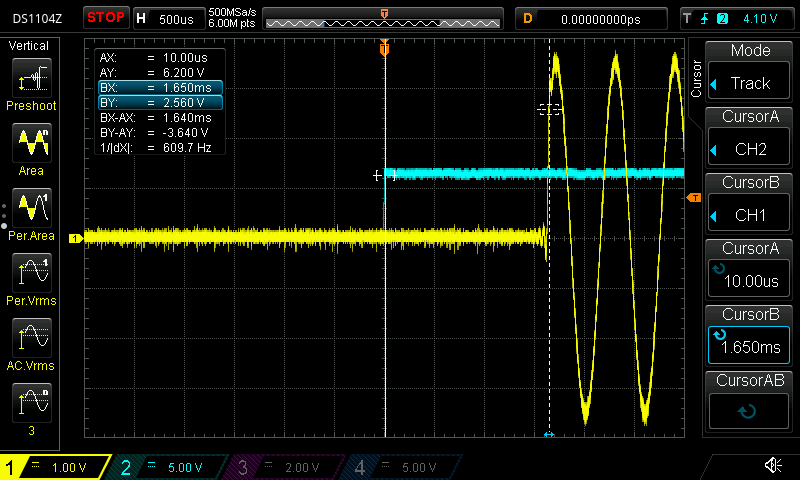
\includegraphics[width=\textwidth]{../images/signal_tests/gate-in_audio_out_latency_tape_enabled/gate-in_audio-out_latency_tape_enabled_07_min_latency.png}
		\subcaption{Minimum measured latency.}
		\label{fig:latency_osc_min}
	\end{minipage}
	\caption{Gate input to audio output latency — oscilloscope captures.}
	\label{fig:latency_osc}
\end{figure}

The measured latency values across all captures are summarised in 
Table~\ref{tab:latency_results}:

\begin{table}[H]
	\centering
	\begin{tabular}{lr}
		\toprule
		\textbf{Measurement} & \textbf{Latency} \\
		\midrule
		Minimum measured     & \qty{1.640}{ms} \\
		Maximum measured     & \qty{2.100}{ms}\\
		Average              & \qty{1.896}{ms} \\
		Std deviation        & \qty{0.144}{ms} \\
		Theoretical maximum  & \qty{4.000}{ms} \\
		\bottomrule
	\end{tabular}
	\caption{Gate-in to audio-out latency measurement results.}
	\label{tab:latency_results}
\end{table}

The measured latency ranges from \qty{1.640}{ms} to \qty{2.100}{ms} across all $n = 19$ measurements, with a mean of \qty{1.896}{ms} and a standard deviation of \qty{0.144}{ms}. 
The peak-to-peak jitter of \qty{0.460}{ms} is well within the theoretical half-block bound of \qty{1.333}{ms}, confirming that command latency is dominated by the block-based processing architecture as expected. 
All measurements fall comfortably within the \qty{10}{ms} perceptual upper bound for gesture-to-audio latency in live performance \cite[p.~13]{davidwesselProblemsProspectsIntimate2002}, as required by the system latency specification (Section~\ref{sec:system-requirements}), with a theoretical worst-case of \qty{4.0}{ms}.
The standard deviation of \qty{0.144}{ms} also falls well within the \qty{1}{ms} jitter tolerance identified by Wessel and Wright~\cite[p.~13]{davidwesselProblemsProspectsIntimate2002}, indicating consistent and predictable timing behaviour across repeated triggers.

\subsubsection{CPU Utilization Measurement}

CPU utilization is measured using the FreeRTOS runtime statistics API in combination 
with the ARM Cortex-M7 \ac{DWT} cycle counter, which increments at the CPU core frequency 
of 280~MHz and serves as the time base for task scheduling measurements. \cite{RunTimeStatistics}
The DWT counter is enabled during system initialization and mapped to the FreeRTOS \texttt{portGET\_RUN\_TIME\_COUNTER\_VALUE} macro, allowing the scheduler to sample elapsed cycles on every context switch.

A delta-based windowed measurement is used rather than lifetime cumulative averages. 
At each measurement interval, \texttt{uxTaskGetSystemState()} is called and per-task utilization is computed as:

\[
	U_i = \frac{\Delta C_i}{\Delta C_{\text{total}}} \times 100\%
\]

where $\Delta C_i$ is the change in cycle count for task $i$ since the previous 
measurement, and $\Delta C_{\text{total}}$ is the change in total runtime over the 
same window.

\paragraph{Results}

Table~\ref{tab:cpu_utilization} summarizes the measured CPU utilization of the audio 
processing task under various processing configurations during active playback and 
recording, averaged over a 5-second window during steady-state operation.

\begin{table}[H]
	\centering
	\begin{tabular}{lc}
		\toprule
		\textbf{Configuration} & \textbf{Audio Task Utilization (\%)} \\
		\midrule
		Full DSP chain (reverb, fades, hermite) & 60--66 \\
		Without Schroeder reverb                & 31--34 \\
		Without reverb and fade processing      & 26--28 \\
		Without reverb, fades, and hermite      & 18--21 \\
		\bottomrule
	\end{tabular}
	\caption{Audio task CPU utilization under varying DSP configurations during 
		playback and recording with cyclic playback fading active.}
	\label{tab:cpu_utilization}
\end{table}

The full DSP chain consumes between 60 and 66\% of total CPU time during active 
playback and recording. The remaining 34--40\% is attributed to the idle task, 
indicating sufficient headroom for the current feature set. The control interface 
and user interface tasks consistently measured at 0\%, as both are notification-driven 
and spend the vast majority of their time blocked.

\paragraph{Per-Stage Cost Analysis}

By selectively disabling individual processing stages the computational cost of 
each stage was isolated, as summarized in Table~\ref{tab:stage_cost}.

\begin{table}[H]
	\centering
	\begin{tabular}{lc}
		\toprule
		\textbf{Processing Stage} & \textbf{Approximate CPU Cost (\%)} \\
		\midrule
		Schroeder stereo reverb      & 28--32 \\
		Hermite interpolation        & 7--9   \\
		Fade processing              & 5--6   \\
		Remaining (tape, exciter)    & 18--21 \\
		\bottomrule
	\end{tabular}
	\caption{Approximate per-stage CPU cost derived from incremental disabling 
		of processing stages.}
	\label{tab:stage_cost}
\end{table}

The Schroeder stereo reverb is the dominant processing cost, accounting for 
approximately half of the total audio task utilization, as it evaluates multiple 
allpass and comb filter stages per sample across both stereo channels at the full 
48~kHz sample rate.

\paragraph{Optimization Proposals}

The per-stage analysis identifies the Schroeder reverb as the primary candidate for optimization. 
Downsampling the reverb input to 24~kHz, processing at half the sample rate, and upsampling the output back to 48~kHz would halve the number of filter evaluations per second. 
Given the perceptually diffuse nature of reverb tails, the resulting reduction in high-frequency content could be acceptable in practice, and reduce total audio task utilization to approximately 30--36\% under full DSP load.

The gained performance can be used to implement more DSP features, like grain-synthesis or experimental filtering.

\subsubsection{Calibration Accuracy}

To verify that the V/Oct input and digital processing chain correctly map CV signals to pitch, a calibration routine has been implemented (see Section~\ref{sec:calibration-and-pitch-tracking}).

\paragraph{Measurement Setup}

The full signal chain -- from CV input through ADC digitization to pitch-controlled playback -- was verified through the following measurement:

\begin{enumerate}
    \item Run the ADC V/Oct boot calibration routine using a calibrated voltage reference.
    \item Record a \SI{1}{kHz} sine wave test signal to the device.
    \item Disable the pitch potentiometer in software to eliminate ADC interference.
    \item Play back the test signal at speeds controlled via the V/Oct CV input.
    \item Verify that $+\SI{1}{V}$ produces a doubling of output frequency, per the V/Oct standard.
\end{enumerate}

\paragraph{Equipment}

Reference voltages were generated with an EA-PS 3016-05 power supply and measured with an OWON XDM1241 multimeter~\cite{owonXDM1000SeriesDatasheet}; output frequency was measured with a Tektronix TBS2000B oscilloscope~\cite{TBS2000BSpecificationVerification_077153803_RevD}.
The combined measurement uncertainty is negligible relative to the deviations under investigation.

\paragraph{Results}

Calibration was performed at \SI{1}{V} and \SI{3}{V} reference points.
Measured voltages deviated by at most \SI{0.5}{mV} from target, within instrument uncertainty (Table~\ref{tab:calibration-voltages}).

\begin{table}[h]
    \centering
    \begin{tabular}{llll}
        \toprule
        \textbf{Point} & \textbf{Target} & \textbf{Meas. 1} & \textbf{Meas. 2} \\
        \midrule
        C1 & $1.0000\,\text{V}$ & $0.9997\,\text{V}$ & $0.9999\,\text{V}$ \\
        C3 & $3.0000\,\text{V}$ & $2.9997\,\text{V}$ & $2.9995\,\text{V}$ \\
        \bottomrule
    \end{tabular}
    \caption{Reference voltages during V/Oct calibration, measured with the OWON XDM1241.}
    \label{tab:calibration-voltages}
\end{table}

V/Oct tracking accuracy was assessed across the operating range with eight frequency measurements per voltage step.

\begin{table}[H]
    \centering
    \begin{tabular}{
            S[table-format=+1.4]
            S[table-format=6.1]
            S[table-format=6.1]
            S[table-format=+3.1]
            S[table-format=+2.2]}
        \toprule
        {Voltage [V]} & {Expected [Hz]} & {Mean [Hz]} & {Dev [Hz]} & {Dev [cents]} \\
        \midrule
        -1.0003 &   499.9 &   499.6 &  -0.3 &  -1.11 \\
        +0.0000 &  1000.0 &  1000.5 &  +0.5 &  +0.78 \\
        +0.9995 &  1999.3 &  1997.6 &  -1.6 &  -1.43 \\
        +2.0002 &  4000.4 &  3994.1 &  -6.3 &  -2.72 \\
        +2.9996 &  7997.8 &  7990.6 &  -7.2 &  -1.55 \\
        +4.0001 & 16001.0 & 16053.8 & +52.8 &  +5.70 \\
        \bottomrule
    \end{tabular}
    \caption{V/Oct tracking accuracy. with expected frequency.}
    \label{tab:voct-results}
\end{table}

The expected frequency is derived from:

\[
f_\text{exp}(U) = 1000 \cdot 2^{U}
\]

Across \SIrange{-1}{+3}{V}, deviations remain within $\pm3\,\text{cents}$, well below the just-noticeable difference for pitch, which is approximately one-twelfth of a semitone ($\approx \qty{8}{cent}$) at the frequencies under investigation~\cite[p.~123]{wheelerScienceSound2014}.
At \SI{4}{V} the deviation rises to $5.70\,\text{cents}$, consistent with degraded interpolation accuracy at the boundary of the calibrated range.
Overall, the V/Oct calibration achieves accurate and deterministic pitch tracking across the primary operating range, with deviations remaining below the perceptual threshold.